%-*- coding=utf-8 -*-
\documentclass[UTF8]{ctexart}
\usepackage{geometry}
\CTEXsetup[format={\Huge\bfseries}]{section}
\CTEXsetup[format={\LARGE\bfseries}]{subsection}
%\usepackage{titlesec}
\geometry{left=3.18cm,right=3.18cm,top=2.54cm,bottom=2.54cm}
\usepackage{graphicx}
\pagestyle{plain}	
% \usepackage{booktabs}
% \usepackage{subfigure}
\usepackage{setspace}
\usepackage{float}
\begin{document}
	\begin{center}
		\quad \\
		\quad \\
		\heiti \fontsize{45}{17} 高级网络编程
		\vskip 2.0cm
		\heiti \fontsize{39}{17} 实验报告	
	\end{center}
	\vskip 3.5cm
	\begin{quotation}
		\par\setlength\parindent{8.5em}
		\quad 
		\heiti 
		
		实验名称:UDP C/S结构程序的开发、uping程序解析
		
		实验日期:2020年5月13日
	
		学生姓名:黄文政
		
		学\hspace{0.72cm}号:71Y17111
		
		\vskip 2cm
		\centering
	\end{quotation}
	
\newpage
\songti \fontsize{13}{13}
\large
\section*{一、实验目的}

1. 掌握UDP C/S结构程序的开发

2. 弄懂ping指令的原理,编写一个ping程序

\section*{二、实验环境}
ubuntu 18.04 LTS

\section*{三、实验内容}
\subsection*{\textbf{UDP C/S结构程序的开发}}
\subsection*{1.设计思路}
本次实验以回射程序为例进行UDP C/S结构的程序开发。(代码参照课件)

对于客户端,首先构造sockaddr\_in,设置好协议族、服务器的IP地址、端口等信息;其次创建一个套接口,并
将套接口类型指定为SOCK\_DGRAM,表示使用UDP;然后在接收到终端的输入内容后,使用SendTo函数将内容发送
至服务器;最后使用Recvfrom接收服务器的回射,并打印内容。

\begin{figure}[H]
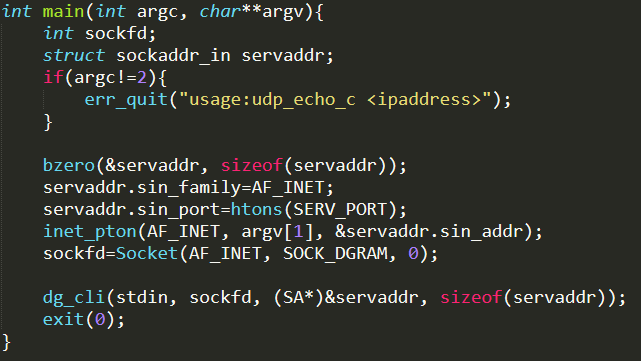
\includegraphics[width=\textwidth]{pic/udp_client_main.PNG}
\caption{UDP客户端部分代码}
\end{figure}

\begin{figure}[H]
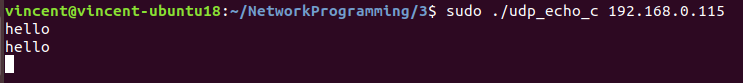
\includegraphics[width=\textwidth]{pic/udp_client.PNG}
\caption{UDP客户端运行结果}
\end{figure}

对于服务端,同样构造sockaddr\_in,设置好协议族、端口等信息;创建一个使用UDP通信的套接口;其次使用
bind()函数将套接口和sockaddr\_in进行绑定,让该套接口对指定端口进行监听;接着使用Recvfrom()函数接
收客户端发来内容;最后将收到的内容通过SendTo()函数进行反射。

\begin{figure}[H]
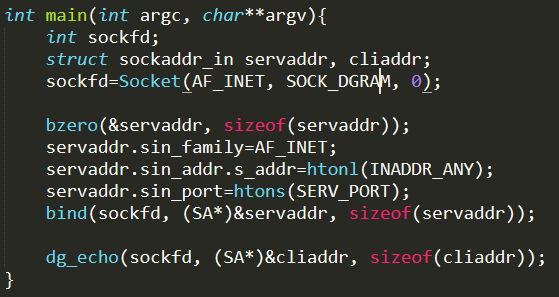
\includegraphics[width=\textwidth]{pic/udp_server_main.PNG}
\caption{UDP服务端部分代码}
\end{figure}

\begin{figure}[H]
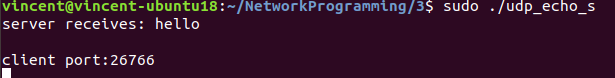
\includegraphics[width=\textwidth]{pic/udp_server.PNG}
\caption{UDP服务器运行结果}
\end{figure}

\par

\subsection*{\textbf{uping程序解析}}
\subsection*{1.设计思路}
uping程序流程介绍:

1.读取输入的IP地址,若为域名,则通过gethostbyname()获取对应的IP地址。

2.使用上一步的IP地址构建sockaddr\_in,准备发送ICMP报文。

3.分别构建三个ICMP数据包,并设置icmp\_seq为1、2、3,将icmp\_id设置为main函数的进程号,发送ICMP包。

4.根据icmp\_id的值判断所收到的是否为目标主机返回的数据包,若是则计算并打印出间隔时间、ttl、rtt等信息。

\subsection*{2.运行结果}

\begin{figure}[H]
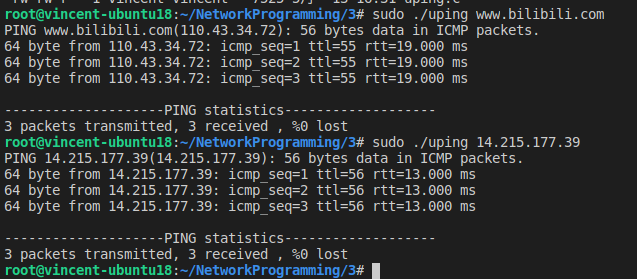
\includegraphics[width=\textwidth]{pic/uping.png}
\caption{uping执行结果}
\end{figure}

\section*{四、实验总结}
在UDP程序开发中,主要遇到的问题是sys/socket.h中sendto的错误,换成unp.h中的Sendto即可。

系统自带的Ping是一种计算机网络工具,用来测试数据包能否透过IP协议到达特定主机。Ping的运作原理是向目标主
机传出一个ICMP的请求回显数据包,并等待接收回显回应数据包。程序会按时间和成功响应的次数估算丢包率和数据
包往返时间(网络时延)。而uping则大体上实现了这样的功能,完成了对ping程序的模拟。

\end{document}